%15 min preso!
\documentclass[xcolor=table,aspectratio=169]{beamer}
\usepackage{beamerthemesplit}
\usepackage{wrapfig}
\usetheme{SPbGU}
\usepackage{pdfpages}
\usepackage{amsmath}
\usepackage{amssymb}
\usepackage{mathtools}
\usepackage{bbm}
\usepackage{cmap}
\usepackage[T2A]{fontenc}
\usepackage[utf8]{inputenc}
\usepackage[english]{babel}
\usepackage{indentfirst}
\usepackage{amsmath}
\usepackage{tikz}
\usepackage{multirow}
\usepackage[noend]{algpseudocode}
\usepackage{algorithm}
\usepackage{algorithmicx}
\usepackage{fancyvrb}
\usepackage{hyperref} 
\definecolor{links}{HTML}{2A1B81}
\hypersetup{colorlinks,linkcolor=,urlcolor=links}
\usetikzlibrary{calc}
\usetikzlibrary{shapes, backgrounds}
\usetikzlibrary{arrows,automata}
\usetikzlibrary{positioning}
\usetikzlibrary{fit}
\usetikzlibrary{shapes.callouts}
\usetikzlibrary{shapes.misc}
\usepackage{xparse}
\usepackage{fontawesome}

\usepackage{etoolbox,refcount}
\usepackage{multicol}
\usepackage[export]{adjustbox}

\usepackage{tabularx}
\newcolumntype{Y}{>{\raggedleft\arraybackslash}X}

\renewcommand{\thealgorithm}{}

\newtheorem{mytheorem}{Theorem}
\renewcommand{\thealgorithm}{}

\newcommand{\tikzmark}[1]{\tikz[overlay,remember picture] \node (#1) {};}
\def\Put(#1,#2)#3{\leavevmode\makebox(0,0){\put(#1,#2){#3}}}

\newcommand{\ltz}{$< 1$}

\tikzset{
    state/.style={
           rectangle,
           rounded corners,
           draw=black, very thick,
           minimum height=2em,
           inner sep=2pt,
           text centered,
           },
}

\tikzset{
    invisible/.style={opacity=0,text opacity=0},
    visible on/.style={alt=#1{}{invisible}},
    alt/.code args={<#1>#2#3}{%
      \alt<#1>{\pgfkeysalso{#2}}{\pgfkeysalso{#3}} % \pgfkeysalso doesn't change the path
    },
}

\tikzset{cross/.style={cross out, draw=black, minimum size=2*(#1-\pgflinewidth), inner sep=0pt, outer sep=0pt, ultra thick},
%default radius will be 1pt. 
cross/.default={1pt}}

\NewDocumentCommand{\mycallout}{r<> O{opacity=0.8,text opacity=1} m m m}{%
\tikz[remember picture, overlay]\node[align=left, fill=cyan!20, text width=#5cm,
#2,visible on=<#1>, rounded corners,
draw,rectangle ]
at (#3) {#4};
}

%\NewDocumentCommand{\mycallout}{r<> O{opacity=0.8,text opacity=1} m m m}{%
%\tikz[remember picture, overlay]\node[align=left, fill=cyan!20, text width=#5cm,
%#2,visible on=<#1>, rounded corners,
%draw,rectangle callout,anchor=pointer,callout relative pointer={(290:0.5cm)}]
%at (#3) {#4};
%}

\NewDocumentCommand{\mycalloutR}{r<> O{opacity=0.8,text opacity=1} m m m}{%
\tikz[remember picture, overlay]\node[align=center, fill=cyan!20, text width=#5cm,
#2,visible on=<#1>, rounded corners,
draw,rectangle callout,anchor=pointer,callout relative pointer={(30:0.8cm)}]
at (#3) {#4};
}


%callout relative pointer={(230:0.5cm)}]

\newcounter{countitems}
\newcounter{nextitemizecount}
\newcommand{\setupcountitems}{%
  \stepcounter{nextitemizecount}%
  \setcounter{countitems}{0}%
  \preto\item{\stepcounter{countitems}}%
}
\makeatletter
\newcommand{\computecountitems}{%
  \edef\@currentlabel{\number\c@countitems}%
  \label{countitems@\number\numexpr\value{nextitemizecount}-1\relax}%
}
\newcommand{\nextitemizecount}{%
  \getrefnumber{countitems@\number\c@nextitemizecount}%
}
\newcommand{\previtemizecount}{%
  \getrefnumber{countitems@\number\numexpr\value{nextitemizecount}-1\relax}%
}
\makeatother    
\newenvironment{AutoMultiColItemize}{%
\ifnumcomp{\nextitemizecount}{>}{3}{\begin{multicols}{2}}{}%
\setupcountitems\begin{itemize}}%
{\end{itemize}%
\unskip\computecountitems\ifnumcomp{\previtemizecount}{>}{3}{\end{multicols}}{}}


\beamertemplatenavigationsymbolsempty

\title[SQL/PGQ for DataFusion]{SQL/PGQ Support in DataFusion}
\institute[SPbSU]{St. Petersburg State University}

% То, что в квадратных скобках, отображается в левом нижнем углу.
\author[Semyon Grigorev]{Semyon Grigorev}

\date{January 15, 2025}


\begin{document}
{
\begin{frame}[fragile]
  \begin{table}
  \centering
  
\includegraphics[height=1cm]{pictures/Untitled.png}
  \vfill
  %\begin{tabularx}{\linewidth}{XcX}
    %\includegraphics[height=1.6cm]{pictures/} 
   % \hfill
   % & 
   % & \hfill 
\includegraphics[height=1.6cm]{pictures/SPbGU_Logo.png}
  %\end{tabularx}
  \end{table}
  \vfill
  \titlepage
\end{frame}
}

\begin{frame}[fragile]
  \frametitle{Semyon Grigorev}
  \begin{minipage}{0.74\textwidth}
  \begin{itemize}    
    \item Research interests:
    \begin{itemize}    
      \item \textbf{Graph analysis} in the context of \textbf{graph databases}
      \item \textbf{Formal language theory} in the context of \textbf{graph querying}
      \item \textbf{Applied linear algebra} in the context of \textbf{graph analysis}
    \end{itemize}
    \item Associate professor at St. Petersburg State University
    \item Email: rsdpisuy@gmail.com 
    \item GitHub: \href{https://github.com/gsvgit}{gsvgit}
    \item Google Scholar: \href{https://scholar.google.com/citations?hl=ru&user=kP4dqUAAAAAJ&view_op=list_works&sortby=pubdate}{Semyon Grigorev}
    \item DBLP: \href{https://dblp.org/pid/181/9903.html}{Semyon V. Grigorev}
  \end{itemize}
\end{minipage}
\begin{minipage}[t]{0.24\textwidth}
  \begin{center}
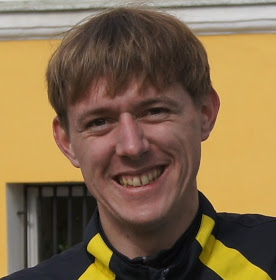
\includegraphics[width=0.8\textwidth]{pictures/SemyonGrigorev.jpg}
  \end{center}
\end{minipage}
\end{frame}

\begin{frame}[fragile]
  \frametitle{Proposal}
  \begin{itemize}
    \item To provide support of PGQ in DataFusion\footnote{Respective \href{https://github.com/apache/datafusion/issues/13545}{issue} on PGQ in DataFusion}
    \begin{itemize}
      \item PGQ is an SQL extension to query \textbf{Property Graphs}
      \item ISO standard: \href{https://www.iso.org/standard/79473.html}{SQL:2023 Part 16: SQL/PGQ --- Property Graph Queries} 
    \end{itemize} 
    \item PGQ adopters
    \begin{itemize}
      \item \href{https://oracle-base.com/articles/23/sql-property-graphs-and-sql-pgq-23}{Oracle}
      \item \href{https://cloud.google.com/spanner/docs/graph/iso-standards}{Google Spanner Graph}
      \item \href{https://github.com/cwida/duckpgq-extension}{DuckDB}
      \item \ldots
    \end{itemize}
  \end{itemize}
\end{frame}


\begin{frame}[fragile]
  \frametitle{Steps}
  \begin{enumerate}
    \item Support PGQ in SQL parser\footnote{Respective \href{https://github.com/apache/datafusion-sqlparser-rs/issues/1572}{issue} on PGQ in sqlparser-rs} 
    \item Improve recursive queries performance\footnote{Related \href{https://github.com/apache/datafusion/issues/462}{issue} on recursive queries in DataFusion with performance issues discussion}
    \begin{itemize}
      \item Ideas from \href{https://dl.acm.org/doi/10.1145/3318464.3380567}{``On the Optimization of Recursive Relational Queries: Application to Graph Queries''} by Louis Jachiet et al.
    \end{itemize}
    \item Translate PGQ to existing building blocks
    \begin{itemize}
      \item It should be possible: \href{https://arxiv.org/abs/2409.01102}{``GQL and SQL/PGQ: Theoretical Models and Expressive Power''} by Amélie Gheerbrant et al.
      \item May be not the most performant solution, but the most straightforward way to the baseline 
    \end{itemize}
    \item Investigate graph-specific techniques
    \begin{itemize}
      \item Indexes
      \item Data structures for data representation
      \item Optimization techniques
    \end{itemize}
    \item Implement graph-specific techniques
  \end{enumerate}
  \tikzmark{xxx}{}
  \mycallout<2>[opacity=1]{$ (xxx) + (11.5,1.4)$}{
    First four steps are (almost) independent
    \begin{itemize}
      \item 1 and 3 share new AST nodes types and related staff
      \item 3 uses results of 2 
      \item At least, 1--4 can be stated in parallel
    \end{itemize}
    }{7.6}
\end{frame}


\begin{frame}[fragile]
  \frametitle{A Bit More on PGQ to Existing Building Blocks Translation}
  \begin{minipage}[t]{0.72\textwidth}
    \begin{itemize}
      \item ``Thus, LCRA\footnotemark \ proposed as the relational processing engine of graph languages like Cypher and GQL is the good old RA in a slight disguise.''\footnotemark
      \item Moreover: ``There are queries that are expressible in positive recursive SQL, and in linear Datalog, and yet are not expressible in Core GQL nor Core PGQ.''\footnotemark
      \pause
      \item Seems that Oracle translates PGQ to SQL and use generic SQL engine\footnotemark
    \end{itemize}
\end{minipage}
\begin{minipage}[t]{0.27\textwidth}
  \pause
  \begin{center}
  
\includegraphics[valign=t,width=0.9\textwidth]{pictures/meme-template.jpeg}
  \end{center}
\end{minipage}
\footnotetext[4]{Linear Composition Relational Algebra}
\footnotetext[5]{``GQL and SQL/PGQ: Theoretical Models and Expressive Power'' by Amélie Gheerbrant et al.}
\footnotetext[6]{Theorem 6.1 from ``GQL and SQL/PGQ: Theoretical Models and Expressive Power''}
\footnotetext[7]{PGQ to SQL query transformation from \href{https://oracle-base.com/articles/23/sql-property-graphs-and-sql-pgq-23\#query-transformation}{``SQL Property Graphs and SQL/PGQ in Oracle Database 23ai''}}
\end{frame}

\setcounter{footnote}{7}

\begin{frame}[fragile]
  \frametitle{A Bit More on Linear Algebra}
    \begin{itemize}
    \item Sparse linear algebra is a promising way to high-performance graph analysis
    \begin{itemize}
      \item \href{https://graphblas.org/}{GrpahBLAS}  --- linear-algebra-based building blocks for graph analysis algorithms
      \begin{itemize}
        \item \href{https://github.com/GraphBLAS/GraphBLAS-Pointers}{GraphBLAS-Pointers} --- collection of GraphBLAS-related materials
        \item \href{https://github.com/DrTimothyAldenDavis/GraphBLAS}{SuiteSparse:GraphBLAS} --- reference implementation in pure C
      \end{itemize}
      \item \href{https://github.com/FalkorDB/falkordb}{FalkorDB} --- linear-algebra-based graph database
      \item \href{https://duckdb.org/}{DuckDB}\footnote{\href{https://www.cidrdb.org/cidr2023/papers/p66-wolde.pdf}{``DuckPGQ:Efficient Property Graph Queries in an analytical RDBMS''} by Daniel ten Wolde et al.} --- column-oriented BD that uses matrix-based representation of graphs for PGQ
    \end{itemize}
    \pause
    \item Not only graphs: mixing of Relational and Linear Algebras is a way to analytical queries
    \begin{itemize}
      \item \href{https://github.com/sandialabs/TenSQL}{TenSQL}\footnote{\href{https://ieeexplore.ieee.org/abstract/document/10363601}{TenSQL: An SQL Database Built on GraphBLAS} by Jon Roose et al.} --- RDBMS that uses sparse linear algebra to execute SQL queries
      \item \href{https://www.sciencedirect.com/science/article/pii/S2772485924000139}{``TensorTable: Extending PyTorch for mixed relational and linear algebra pipelines''} by Xu Wen  et al.
      \item \href{https://dl.acm.org/doi/abs/10.1145/3514221.3517869}{TCUDB: Accelerating Database with Tensor Processors} by Yu-Ching Hu  et al. % SIGMOD 2022
      \item \href{https://dl.acm.org/doi/abs/10.1145/3318464.3389747}{A Relational Matrix Algebra and its Implementation in a Column Store}  by Oksana Dolmatova  et al. %SIGMOD 2020
    \end{itemize}
  \end{itemize}
\end{frame}

\begin{frame}[fragile]
  \frametitle{Qustions to Discuss}
  \begin{enumerate}
    \item PGQ integration ways
    \begin{itemize}
      \item Oracle-like way: $\overbrace{PGQ \to SQL}^{\mathclap{\text{new AST-level transformation}}} \underbrace{\to \ldots}_{\mathclap{\text{existing pipeline}}}$
      \item Alternative way: $\overbrace{SQL+PGQ}^{\mathclap{\text{extended existing AST}}} \xrightarrow[\text{existing translator}]{\text{extended}} \underbrace{\text{logical plan} \to \ldots}_{\mathclap{\text{existing pipeline}}} $
      \item Other ideas?
    \end{itemize}
  \tikzmark{xxx}{}
  \mycallout<2->[opacity=1]{$ (xxx) + (10.8,3.2)$}{
    What one should we choose?  
  \begin{itemize}
      \item First one is easier to implement
      \item Second one (possibly) allows for fine-grained optimizations
    \end{itemize}
    }{6.6}
    \onslide<3>{
    \item Linear algebra
    \begin{itemize}
      \item Is it in the scope of te community?
      \item If yes, what direction is preferable?      
    \end{itemize}
    \item Other advanced techniques for PGQ/graphs
    \begin{itemize}
      \item Is it in the scope of te community?
      \item If yes, what direction is preferable?
    \end{itemize}
    }
  \end{enumerate}
\end{frame}


\end{document}
